\documentclass[12pt]{article}

\usepackage[margin=1in, headheight=14.5pt]{geometry}
\usepackage{graphicx}
\usepackage{booktabs}
\usepackage{listings}
\usepackage{xcolor}
\usepackage{amsmath,amssymb}
\usepackage{caption}
\usepackage{float}
\usepackage{hyperref}
\usepackage{enumitem}
\usepackage{tabularx}
\usepackage{adjustbox}
\usepackage{fancyhdr}
\usepackage{titling}
\usepackage{indentfirst}
\usepackage[numbers]{natbib}

\setlength{\parindent}{1.5em}

\hypersetup{
  colorlinks=true,
  linkcolor=blue!60!black,
  urlcolor=blue!60!black,
  citecolor=blue!60!black,
}

% Page header/footer
\pagestyle{fancy}
\fancyhf{}
\fancyhead[L]{\small ECEC661 --- Homework 2}
\fancyhead[R]{\small Gary Pham (gp492)}
\fancyfoot[C]{\thepage}
\renewcommand{\headrulewidth}{0.4pt}

% C listing style (matches the VHDL colour palette used in Homework~1)
\definecolor{ckw}{RGB}{0,0,180}
\definecolor{ccmt}{RGB}{0,128,0}
\definecolor{cstr}{RGB}{160,0,0}
\definecolor{codebg}{RGB}{245,245,248}

\lstdefinestyle{cstyle}{
  language=C,
  morekeywords={u32,u16,u8,UINTPTR,XGpio,XGpio_Config,XStatus},
  basicstyle=\ttfamily\footnotesize,
  keywordstyle=\color{ckw}\bfseries,
  commentstyle=\color{ccmt}\itshape,
  stringstyle=\color{cstr},
  backgroundcolor=\color{codebg},
  frame=single,
  framerule=0.4pt,
  rulecolor=\color{gray!50},
  numbers=left,
  numberstyle=\tiny\color{gray},
  numbersep=6pt,
  breaklines=true,
  showstringspaces=false,
  tabsize=4,
  captionpos=b,
  aboveskip=8pt,
  belowskip=4pt,
}
\lstset{style=cstyle}

% Title configuration
\pretitle{\begin{center}\LARGE\bfseries}
\posttitle{\par\end{center}\vskip 0.3em}

\title{ECEC661 --- Homework 2\\
       \large Running-LED Application on the Digilent Cora Z7-07S}
\author{Gary Pham --- gp492}
\date{\today}

\begin{document}
\maketitle
\thispagestyle{fancy}

% ======================================================================
\begin{abstract}
This report documents an embedded application that drives a six-channel
running-LED display on the Digilent Cora Z7-07S
board~\cite{coraz7rm}, using the Zynq-7000S Processing System as the
host and two AXI~GPIO cores in the Programmable Logic as the
peripherals. The application sweeps a single-bit window across the six
RGB-LED channels and lets the user toggle the direction of the sweep
via the two on-board push-buttons. The Vivado block design, the Xilinx
Design Constraints (XDC) pin mapping, and the bare-metal C application
compiled in Vitis Unified 2025.2 are presented. Verification was
carried out on hardware: pressing \texttt{BTN1} selects the R--G--B
(left-to-right) colour sweep and \texttt{BTN0} selects the B--G--R
(right-to-left) colour sweep, both running at a 500\,ms step interval.
\end{abstract}

% ======================================================================
\section{Problem Statement}
\label{sec:problem}
% ======================================================================

Code an application that displays a running LED left-to-right or
right-to-left when a button is toggled. The implementation is to run on
a Xilinx Zynq-7000 based development board using a Processing System
(PS) plus Programmable Logic (PL) flow: the PL provides the AXI~GPIO
peripherals that map external pins into the PS memory map, and the PS
runs a bare-metal C application that drives those peripherals.

\paragraph{Deliverables.}
\begin{itemize}[nosep]
  \item Snipped image of the Vivado IP-integrator block diagram
        (Figure~\ref{fig:bd}).
  \item C application source code
        (Listing~\ref{lst:led}).
  \item Live demo (in class) or recorded video of the running
        application on the board.
\end{itemize}

% ======================================================================
\section{Hardware Platform}
\label{sec:hw}
% ======================================================================

The target board is the Digilent Cora Z7-07S~\cite{coraz7rm}, which
hosts a Xilinx Zynq-7000S (\texttt{xc7z007sclg400-1}) SoC with a
single-core ARM Cortex-A9 application processor and a small
Artix-7-equivalent programmable fabric. The board exposes two
push-buttons (\texttt{BTN0}, \texttt{BTN1}) and two tri-colour RGB LEDs
(\texttt{LD0}, \texttt{LD1}); each LED exposes three independently
driven colour pins, for a total of six LED channels. All eight signals
are \texttt{LVCMOS33} and are active-high.

\subsection{Block Diagram}
\label{sec:bd}

Figure~\ref{fig:bd} shows the Vivado~2025.2 IP-integrator block design.
The ZYNQ~Processing System exports a single \texttt{M\_AXI\_GP0}
interface clocked at 50\,MHz (from \texttt{FCLK\_CLK0}). An
AXI~SmartConnect fans this out to two AXI~GPIO cores:

\begin{itemize}[nosep]
  \item \texttt{axi\_gpio\_0}~\cite{pg144} --- 6-bit, all-outputs,
        mapped to the external interface
        \texttt{rgb\_leds\_tri\_o[5:0]} and wired to the six RGB-LED
        pins. Base address \texttt{0x41200000}.
  \item \texttt{axi\_gpio\_1} --- 2-bit, all-inputs, mapped to the
        external interface \texttt{btns\_2bits\_tri\_i[1:0]} and wired
        to the two push-button pins. Base address \texttt{0x41210000}.
\end{itemize}

\noindent
The Processor System Reset block (\texttt{rst\_ps7\_0\_50M})
synchronises the global reset with the AXI clock, driving
\texttt{peripheral\_aresetn} to every AXI slave.

\begin{figure}[H]
  \centering
  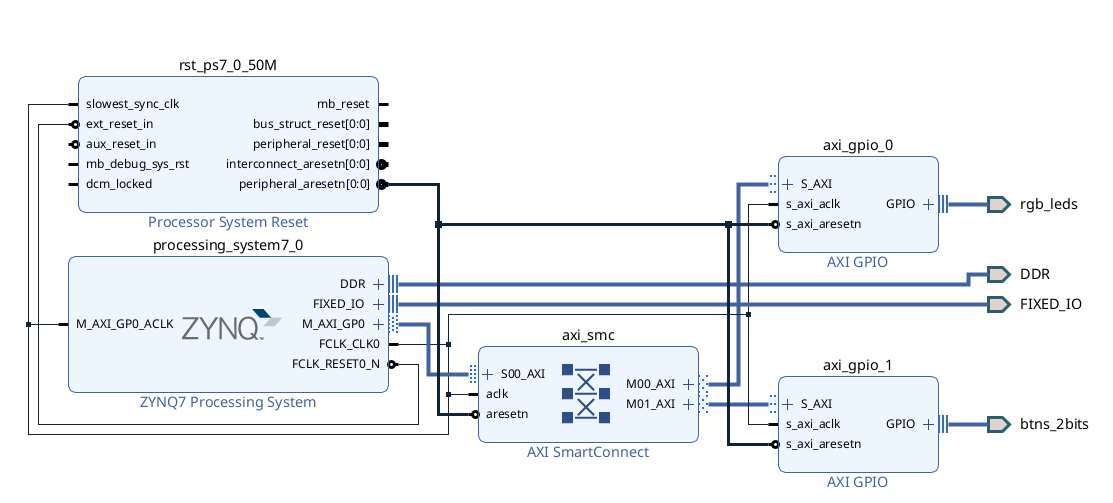
\includegraphics[width=\textwidth]{Diagram.png}
  \caption{Vivado IP-integrator block design for the running-LED
           application. The Zynq~PS drives two AXI~GPIO cores via an
           AXI~SmartConnect: one for the six RGB-LED output channels
           and one for the two push-button inputs.}
  \label{fig:bd}
\end{figure}

\subsection{Pin Assignment (XDC)}
\label{sec:xdc}

The six LED bits and two button bits were assigned in a user XDC file
derived from Digilent's official
\texttt{Cora-Z7-07S-Master.xdc}~\cite{coraz7master}. The bit-to-pin
mapping is listed in Table~\ref{tab:xdc}.

\begin{table}[H]
\centering
\caption{Pin assignment for the external ports. All pins are
         \texttt{LVCMOS33}.}
\label{tab:xdc}
\begin{tabular}{@{}llll@{}}
\toprule
\textbf{Top-level port} & \textbf{Package pin} & \textbf{Board net} & \textbf{Role} \\
\midrule
\texttt{rgb\_leds\_tri\_o[0]}  & \texttt{N15} & \texttt{led0\_r} & LD0 Red   \\
\texttt{rgb\_leds\_tri\_o[1]}  & \texttt{G17} & \texttt{led0\_g} & LD0 Green \\
\texttt{rgb\_leds\_tri\_o[2]}  & \texttt{L15} & \texttt{led0\_b} & LD0 Blue  \\
\texttt{rgb\_leds\_tri\_o[3]}  & \texttt{M15} & \texttt{led1\_r} & LD1 Red   \\
\texttt{rgb\_leds\_tri\_o[4]}  & \texttt{L14} & \texttt{led1\_g} & LD1 Green \\
\texttt{rgb\_leds\_tri\_o[5]}  & \texttt{G14} & \texttt{led1\_b} & LD1 Blue  \\
\texttt{btns\_2bits\_tri\_i[0]} & \texttt{D20} & \texttt{btn[0]}  & BTN0 \\
\texttt{btns\_2bits\_tri\_i[1]} & \texttt{D19} & \texttt{btn[1]}  & BTN1 \\
\bottomrule
\end{tabular}
\end{table}

% ======================================================================
\section{Software Design}
\label{sec:sw}
% ======================================================================

The application is a bare-metal C program that runs on the
Cortex-A9 core and uses the standalone BSP generated by
Vitis~Unified~2025.2 from the exported
\texttt{system\_wrapper.xsa}~\cite{ug1400}. It relies on two drivers:

\begin{itemize}[nosep]
  \item \texttt{xgpio} --- Xilinx AXI~GPIO driver; offers
        \texttt{XGpio\_Initialize}, \texttt{XGpio\_SetDataDirection},
        \texttt{XGpio\_DiscreteWrite}, and
        \texttt{XGpio\_DiscreteRead}.
  \item \texttt{xil\_printf} --- lightweight \texttt{printf}-family
        routine that sends formatted output to the PS UART for
        debugging.
\end{itemize}

\subsection{Control-Flow Description}

After initialising the platform and both AXI~GPIO instances, the
program configures channel~1 of the LED GPIO as all-outputs
(direction register = \texttt{0x00}) and channel~1 of the button GPIO
as all-inputs (direction register = \texttt{0xFF}). Two
compile-time constant tables select the colour-walk order across the
six LED channels:

\begin{itemize}[nosep]
  \item \texttt{seq\_rgb = \{0,1,2,3,4,5\}} --- R$\rightarrow$G$\rightarrow$B
        within \texttt{LD0}, then R$\rightarrow$G$\rightarrow$B within
        \texttt{LD1} (left-to-right order).
  \item \texttt{seq\_bgr = \{2,1,0,5,4,3\}} --- B$\rightarrow$G$\rightarrow$R
        within \texttt{LD0}, then B$\rightarrow$G$\rightarrow$R within
        \texttt{LD1} (right-to-left order).
\end{itemize}

\noindent
Inside the main loop the program writes a one-hot mask
\texttt{(1U << seq[idx]) \& LED\_MASK} to the LED register, delays
\texttt{STEP\_DELAY\_US = 500\,ms}, then polls the button register and
switches the active sequence table:

\begin{itemize}[nosep]
  \item \texttt{BTN1} asserted $\Rightarrow$ switch to \texttt{seq\_rgb}
        (left-to-right),
  \item \texttt{BTN0} asserted $\Rightarrow$ switch to \texttt{seq\_bgr}
        (right-to-left).
\end{itemize}

\noindent
A state-change print (\texttt{Mode:\ RGB} / \texttt{Mode:\ BGR}) is
emitted only on transitions, so the UART is not flooded while a button
is held. The counter \texttt{idx} is incremented modulo \texttt{LED\_COUNT}
on every step so that the active sequence is walked cyclically.

\subsection{Source Listing}

\lstinputlisting[
  caption={\texttt{led.c} --- Bare-metal running-LED application.},
  label={lst:led}
]{../workspace/led_control_rgb/src/led.c}

% ======================================================================
\section{Verification and Demonstration}
\label{sec:verify}
% ======================================================================

The application was built and deployed as follows:

\begin{enumerate}[nosep]
  \item Vivado~2025.2: synthesise, implement, and write the bitstream
        for the block design in Figure~\ref{fig:bd}. Export the
        hardware (including bitstream) to
        \texttt{system\_wrapper.xsa}.
  \item Vitis~Unified~2025.2: create a platform from the XSA, create
        an empty standalone application \texttt{led\_control\_rgb},
        add \texttt{led.c}, and build.
  \item Launch the debugger; the launcher programs the PL with
        \texttt{system\_wrapper.bit} and downloads the ELF to the
        Cortex-A9 core.
\end{enumerate}

\noindent
On power-up the LEDs start in left-to-right (RGB) mode. Observed
behaviour matches the specification:

\begin{itemize}[nosep]
  \item One colour channel is lit per 500\,ms step.
  \item Pressing \texttt{BTN1} starts (or keeps) the sweep in R$\rightarrow$G$\rightarrow$B order
        across \texttt{LD0} then \texttt{LD1}.
  \item Pressing \texttt{BTN0} flips the sweep to B$\rightarrow$G$\rightarrow$R order.
  \item The UART console prints \texttt{Mode:\ RGB} and
        \texttt{Mode:\ BGR} on each transition, which is useful for
        confirming button inputs reach the application.
\end{itemize}

\paragraph{Video demonstration.}
A short video of the running application on hardware is available on
Drexel MediaSpace~\cite{demovideo}:

\begin{center}
\href{https://1513041.mediaspace.kaltura.com/media/ECEC+661+-+SP+25+26+-+Homework+2+-+LED+Control+-+Gary+Pham/1_m3jcfnvb}%
     {\textbf{ECEC 661 --- SP 25/26 --- Homework 2 --- LED Control --- Gary Pham}}
\end{center}

\noindent
The video shows the board powering up in left-to-right (RGB) mode,
\texttt{BTN0} flipping the sweep to right-to-left (BGR) mode, and
\texttt{BTN1} restoring left-to-right mode, with the UART console
reporting each transition.

% ======================================================================
\section{Conclusion}
\label{sec:conclusion}
% ======================================================================

A Zynq-7000S based running-LED application was built end-to-end on the
Cora Z7-07S board. The Vivado block design exposes six LED outputs and
two push-button inputs through two AXI~GPIO cores; the user XDC maps
them to the correct board pins at \texttt{LVCMOS33}. A bare-metal C
application running on the Cortex-A9 core sweeps a one-hot mask across
the six LED channels and switches between left-to-right (RGB) and
right-to-left (BGR) sweep orders based on the pressed button.
Functional correctness was verified on hardware: both sweep directions
are selectable from the two on-board push-buttons, and the transition
is reported over UART for convenience.

% ======================================================================
% References
% ======================================================================
\bibliographystyle{ieeetr}

\begin{thebibliography}{9}

\bibitem{coraz7rm}
Digilent, ``Cora Z7 Reference Manual,''
\url{https://digilent.com/reference/programmable-logic/cora-z7/reference-manual}

\bibitem{coraz7master}
Digilent, ``Cora-Z7-07S-Master.xdc,''
\url{https://github.com/Digilent/digilent-xdc/blob/master/Cora-Z7-07S-Master.xdc}

\bibitem{ug1400}
AMD/Xilinx, ``Vitis Unified Software Platform Documentation: Embedded
Software Development (UG1400),'' v2025.2, 2025.
\url{https://docs.amd.com/r/en-US/ug1400-vitis-embedded}

\bibitem{pg144}
AMD/Xilinx, ``AXI GPIO v2.0 LogiCORE IP Product Guide (PG144),''
2022.
\url{https://docs.amd.com/v/u/en-US/pg144-axi-gpio}

\bibitem{demovideo}
G.~Pham, ``ECEC 661 --- SP 25/26 --- Homework 2 --- LED Control ---
Gary Pham,'' Drexel MediaSpace, 2026.
\url{https://1513041.mediaspace.kaltura.com/media/ECEC+661+-+SP+25+26+-+Homework+2+-+LED+Control+-+Gary+Pham/1_m3jcfnvb}

\end{thebibliography}

\end{document}
